%\pagenumbering{arabic}
%\setcounter{page}{1}
\chapter{The Central Limit Theorem}
%\index{Introduction}
%\label{sec.matrix}
%start relabeling as 2.1 etc
%\pagestyle{myheadings}  \markboth{\ref{sec.matrix}.
%\titleref{sec.matrix}}{}
%\setcounter{equation}{0}

The Central Limit Theorem (CLT) is one of the most important results in probability and statistics. It states that, given a sufficiently large sample size, the distribution of the sample mean of independent and identically distributed (i.i.d.) random variables approaches a normal distribution, regardless of the shape of the original distribution. Real-life Application of Central Limit Theorem in Financial Analysis. The CLT is often used by financial experts to examine stock market results.\\

\noindent
Now, let's discuss Central Limit Theorem with more details. Suppose we have a finite number of populations and each population follows a distribution with population mean $\mu$ and population variance $\sigma^2.$. Then we take samples of same size $n$ from each population, such that we have $\bar{x}_1, \bar{x}_2, ..., \bar{x}_m$ from population group $1 \text{ to } m, \text{ respectively.}$ Next, we make a histogram using the large collection of sample taken from each population group. Then, what we are doing right row is sampling distribution of $\bar{x}$. As a result, $\bar{x}$ follows a normal distribution with mean $\mu_{\bar{x}} = \mu$ and variance $\sigma_{\bar{x}}^{2} = \frac{\sigma^2}{n}$, which is denoted as the following: \[ \bar{x} \sim N(\mu_{\bar{x}} = \mu, \text{ } \sigma_{\bar{x}}^{2} = \frac{\sigma^2}{n}).\]

\noindent
Figure $3.1$ below shows the entire procedure about the Central Limit Theorem. 

\begin{figure}[H]
 \centering
 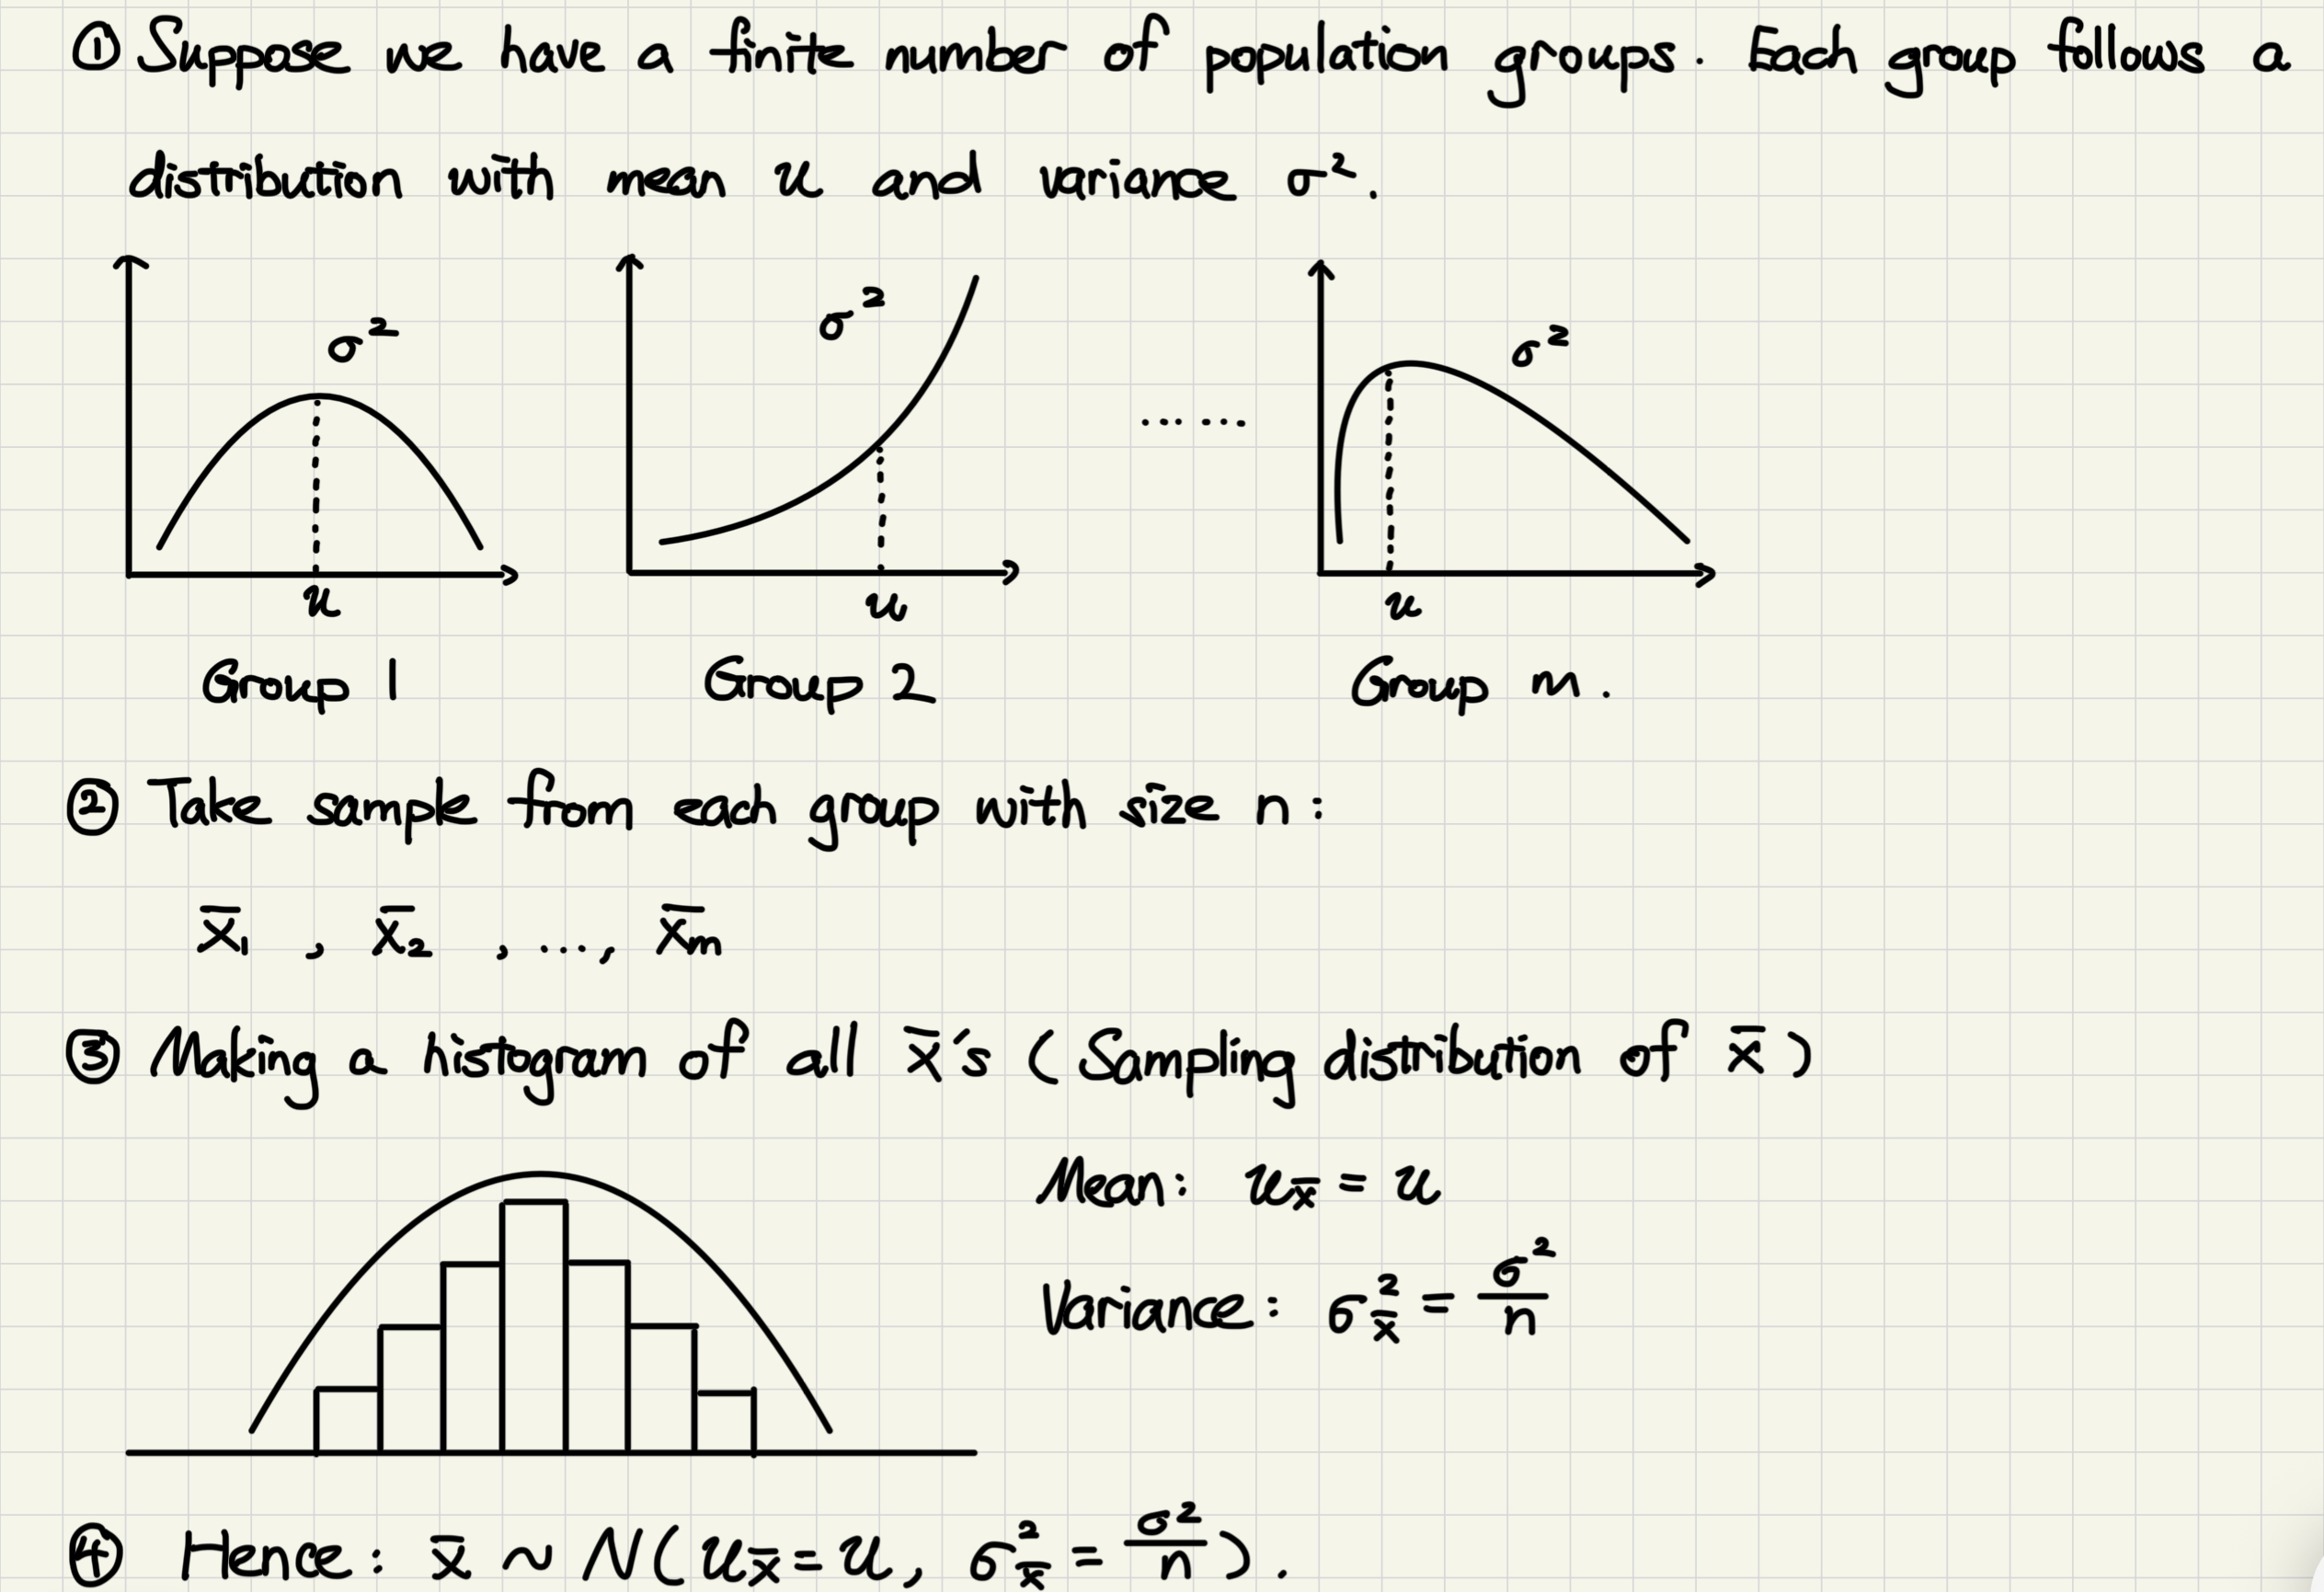
\includegraphics[scale=0.15]{Section3/Img3/CLT.jpg}
 \caption{Procedure of the Central Limit Theorem}
\end{figure}

\noindent
Now, let's begin with the proper definition of Central Limit Theorem.

\begin{definition}[Central Limit Theorem]
Let $X_1, X_2, ..., X_n$ be independent and identically distributed random variables with $E(X_i) = \mu$ and $Var(X_i) = \sigma^2 < \infty$. Then, we define the following: \[ U_{n} = \frac{\bar{X} - \mu}{(\frac{\sigma}{\sqrt{n}})} \sim N(\mu = 0, \sigma^2 = 1), \text{ where $\bar{X} = \frac{1}{n} \sum_{i =1}^{n}X_i$.}\]
Then the distribution function of $U_{n}$ converges to the standard Normal distribution function as $n \longrightarrow \infty$. That is, \[ \lim_{n\to\infty}P(U_n \le u) = \int_{\infty}^{u} \frac{1}{\sqrt{2\pi}} e^{-\frac{t^2}{2}}\,dt; \text{ for all u.}\]
\end{definition}

\noindent
For this course in particular, we do not need to pay that much attention to the proving part of the definition above. However, we use Central Limit Theorem to approximate distributions. Here are the two important approximations:

\begin{itemize}
	\item $\bar{X_n} \approx N(\mu, \frac{\sigma^2}{n});$
	\item $T = \sum_{i = 1}^{n}X_i \approx N(n\mu, n\sigma^2).$
\end{itemize}

\noindent
A reminder that the distribution of $U_n$ in definition $3.1$ and the two approximation of distribution above are extremely important in this course, until later chapters you may see some materials that are similar.